Показательная функция - это монотонно возрастающая функция при $a>0$ и монотонно убывающая при $0<a<1$. Именно этим свойством мы пользуемся при решении уравнений и неравенств. (Как именно?)

\begin{figure}[h!]
	\centering
	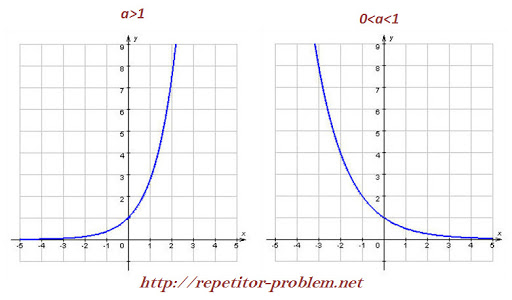
\includegraphics[width=0.7\textwidth]{img/pokaz.jpg}
	\caption{Показательная функция}
\end{figure}